\chapter{Adaptive Optik\label{chapter:thema}}
\lhead{Adaptive Optik}
\begin{refsection}
\chapterauthor{Matthias Schneider}

\section{Einleitung}
In diesem Kapitel wird das Thema Adaptive Optik behandelt, dazu werde ich zuerst eine kurze Übersicht über das Thema geben und anschliessend einige Aspekte genauer erklären. \newline

\section{Adaptive Optik und ihre Anwendungen}
Adaptive Optik (AO) ist eine Technik mit der optische Systeme verbessert werden können. Dabei können aber nur Fehler korrigiert werden, welche im Medium zwischen der Quelle des Lichtes und dem Sensor entstehen, hauptsächlich geht es also darum, Fehler die durch die Atmosphärenunruhe entstehen zu kompensieren. Die erdgebundene Astronomie ist heute auf diese Technologie angewiesen, denn Beobachtungen im optischen und infraroten Bereich sind nur möglich, wenn die negativen Effekte der Atmosphäre korrigiert werden können. Ein schönen Beispiel dazu ist die Abbildung \ref{fig:jupiter}, sie zeigt eine Aufnahme vom Jupiter mit dem Very Large Telescope (VLT) der European Southern Observatory (ESO).
\begin{figure}
  \centering
  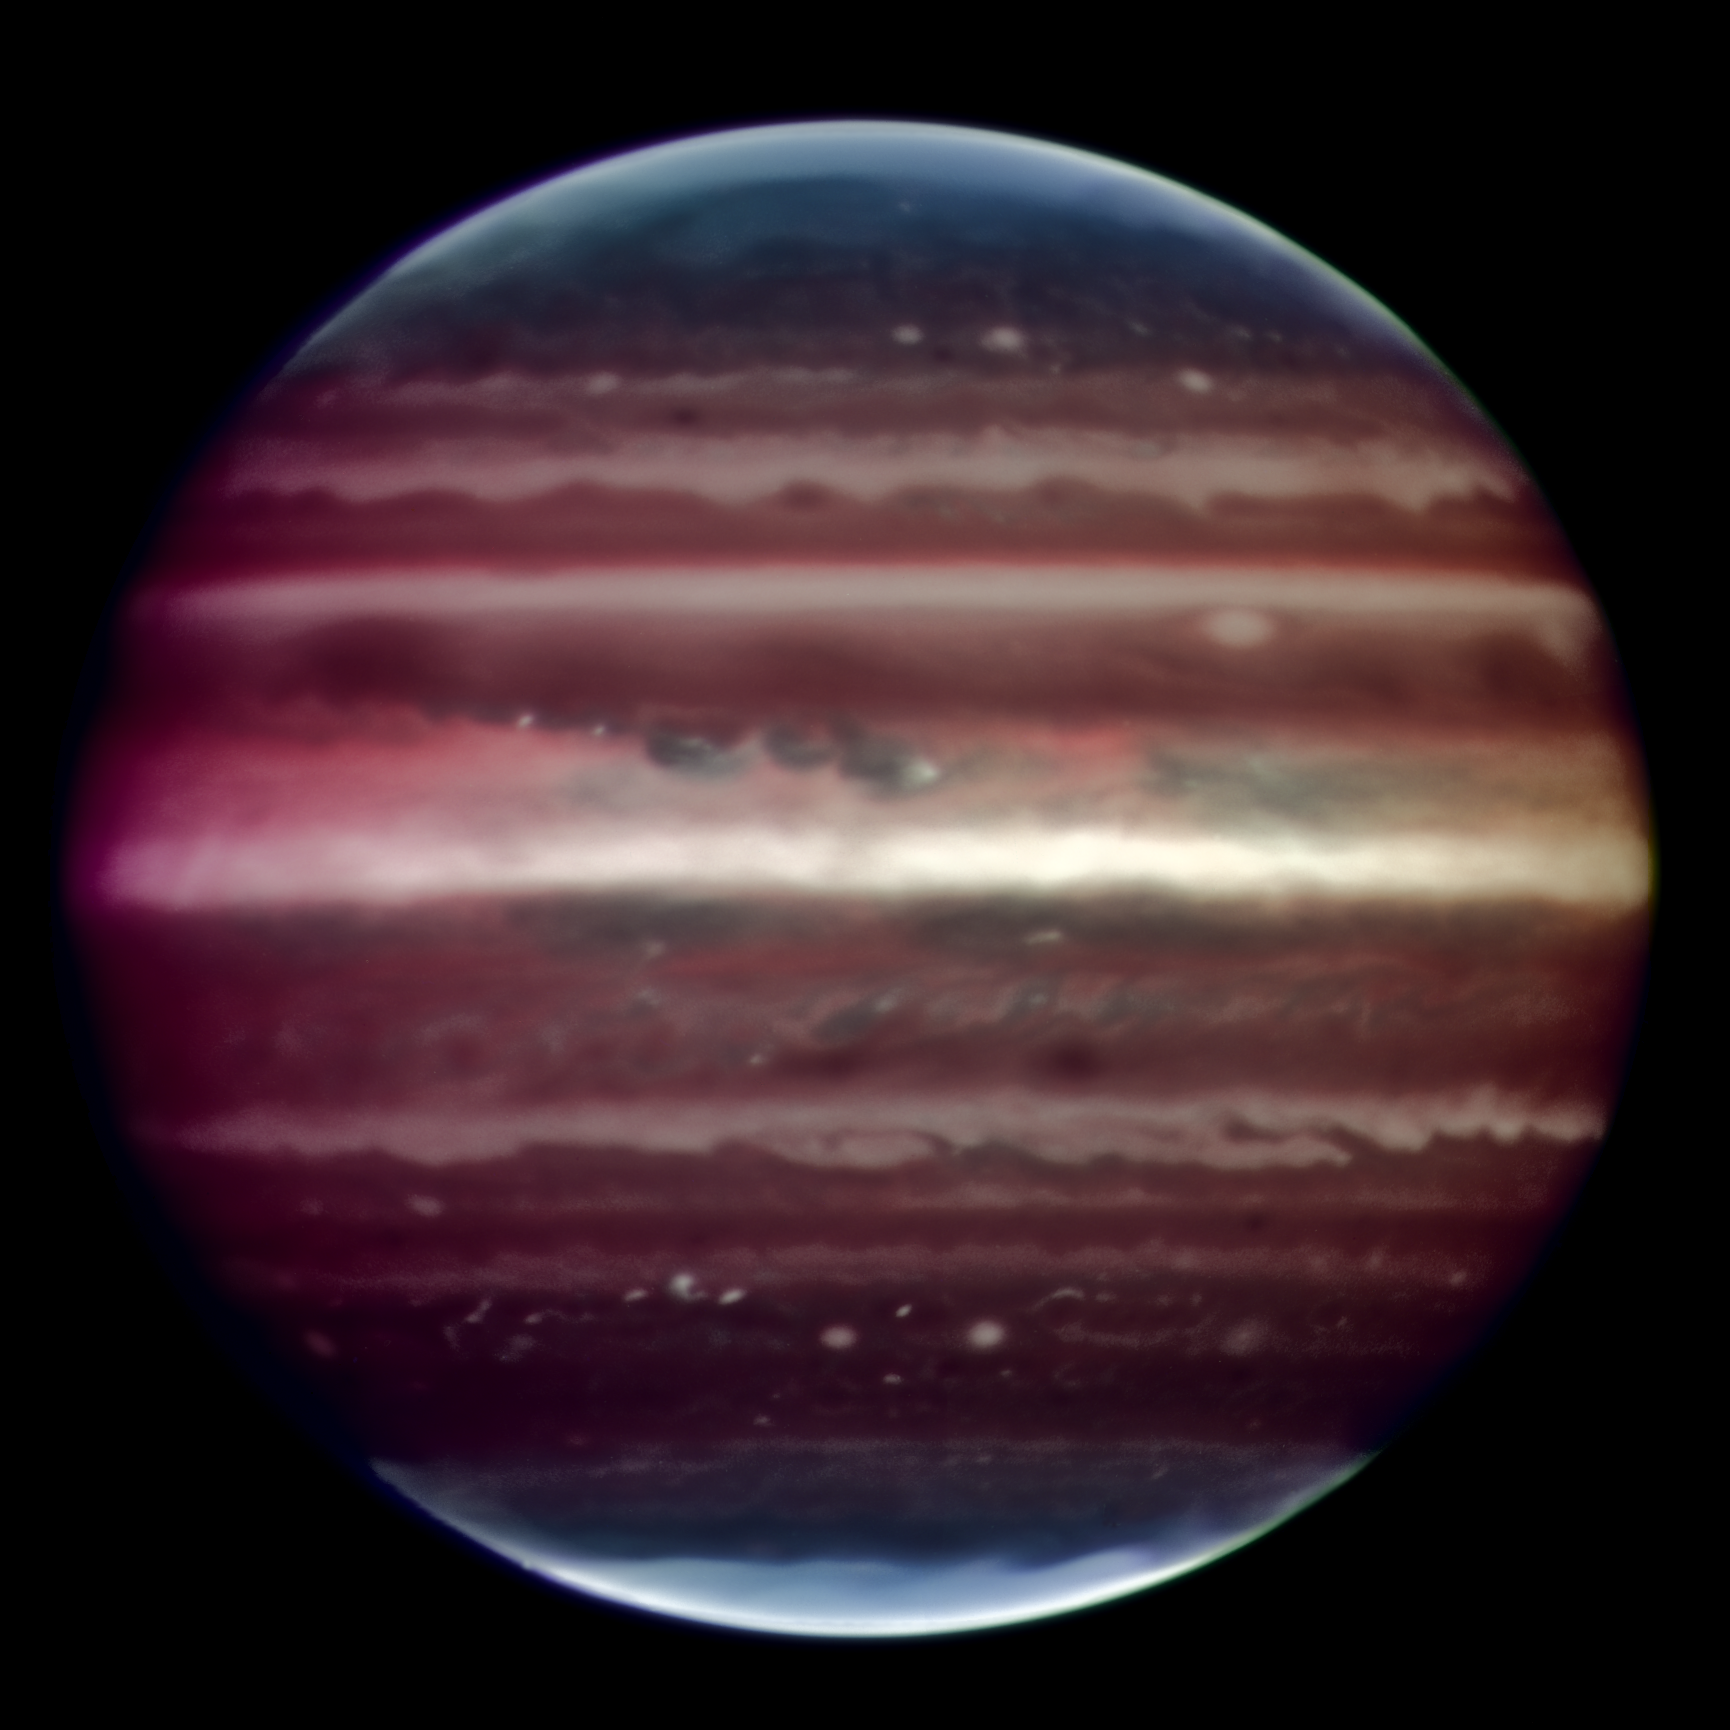
\includegraphics[width=0.5\textwidth]{adaptiv/images/Jupiter_adaptiv}
  \caption{Jupiter mit adaptiver Optik von der Erde aus mit VLT aufgenommen
    \cite{eso:jupiter}}
  \label{fig:jupiter}
\end{figure}
Adaptive Optik wird heute aber auch bei anderen Anwendungen eingesetzt, um die Präzision von Optischen Apparaturen zu erhöhen, so gibt es heute Mikroskope mit AO. Ein weiterer Einsatzbereich dieser Technologie ist der Fokusiserspiegel von Laserschneidanlagen, womit eine deutliche Steigerung der Präzision beim schneiden erreicht werden kann.\newline
Ein System mit einer adaptiven Optik ist aus drei Hauptkomponenten aufgebaut. Es braucht einen Sensor, der die Störung der Wellenfront messen kann, einen Computer der die benötigte Korrektur berechnet und einen beweglichen Spiegel, mit welchem die Wellenfront korrigiert werden kann. So ist es möglich auf den Messinstrument, welchen das Nutzsignal misst, ein möglichst scharfes Bild zu haben, trotz nicht optimalen Bedingungen.\newline
Als Sensor wird für gewöhnlich eine Hartmannplatte verwendet, welche aus einem Mikrolinsenarray besteht und pro Linse einen CMOS oder CCD-Sensor, mit welchem die Verkippung der Wellenfront im Bereich einer einzelnen Linse bestimmt werden kann. Auf der Abbildung \ref{fig:hartmannplatte} ist gut zu erkennen, was geschieht, wenn die Wellenfront nicht mehr eben, sondern durch die Atmosphäre leicht gestört wird. Das Licht des Leitsterns wird nun durch die einzelnen Linsen des Arrays nicht mehr in die Mitte des Sensors fokussiert, sondern leicht verschoben. Diese Verschiebung wird gemessen und daraus die benötigte Korrektur berechnet und damit der bewegliche Spiegle in Stellung gebracht, damit die Wellenfront nahezu ohne Störung der in das Messinstrument geleitet werden kann. Dieser Zyklus auf Störung messen, Korrektur berechnen und Spiegel in Stellung bringen, wird etwas 1000 mal pro Sekunde wiederholt, was auch eine hohe Leistung und Spezialisierung des Korrekturrechners erfordert. Dazu wird oft eine Regelstrecke aufgebaut mit welcher dieser Zyklus geregelt werden kann, auf der Abbildung \ref{fig:schematischAO} ist dieser Regelkreis schematisch dargestellt.

\begin{figure}
  \centering
  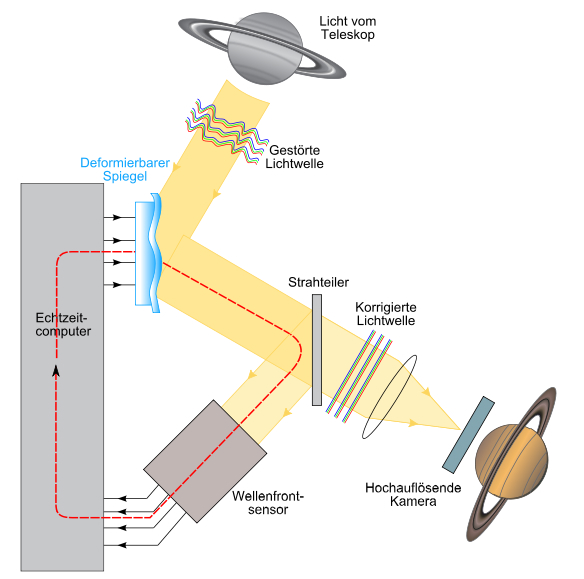
\includegraphics[width=0.6\textwidth]{adaptiv/images/schematichAO}
  \caption{Schematische Darstellung des Regelkreises einer AO
    \cite{robani:schematischAO}}
  \label{fig:schematischAO}
\end{figure}

\begin{figure}
  \centering
  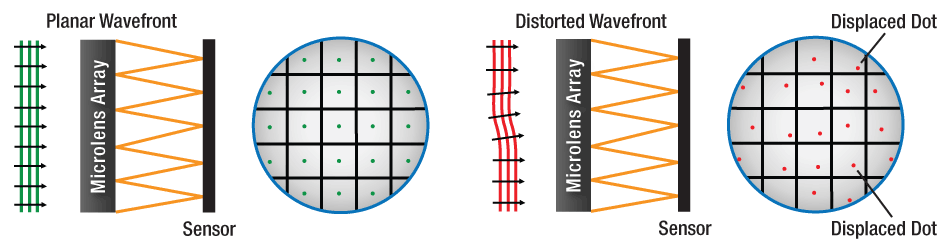
\includegraphics[width=0.9\textwidth]{adaptiv/images/hartmannplatte}
  \caption{Hartmannplatte mit ebener und verformter Wellenfront
    \cite{thor:hartmannplatte}}
  \label{fig:hartmannplatte}
\end{figure}

Ein weiteres wichtiges Element bei der adaptiven Optik ist das Erzeugen einer Referenzquelle, welche ein Signal erzeugt, dass bekannt ist und so der Einfluss der Atmosphäre gemessen werden kann. In der Astronomie wird dazu mit Laser ein künstlicher Stern erzeugt, dieser sogenannte Leitstern. Er wird in einer Höhe von etwa 90$km$ erzeugt, also am oberen Ende der Mesosphäre. Dazu wird oft ein Natrium-Laser verwendet, der eine Wellenlänge von 589$nm$ hat. Dieses Licht wird dann von den Natriumatomen in der Höhe von 90$km$ zurückgeworfen. Dabei wird die Annahme gemacht, dass dabei ein Stern entsteht, dessen Licht sich Kugelförmig ausbreitet wichtig ist dabei, dass der Stern in Beobachtungsrichtung vom Teleskop erzeugt wird, damit nur die Atmosphäre welche störende Einflüsse hat gemessen wird. 

\begin{figure}
  \centering
  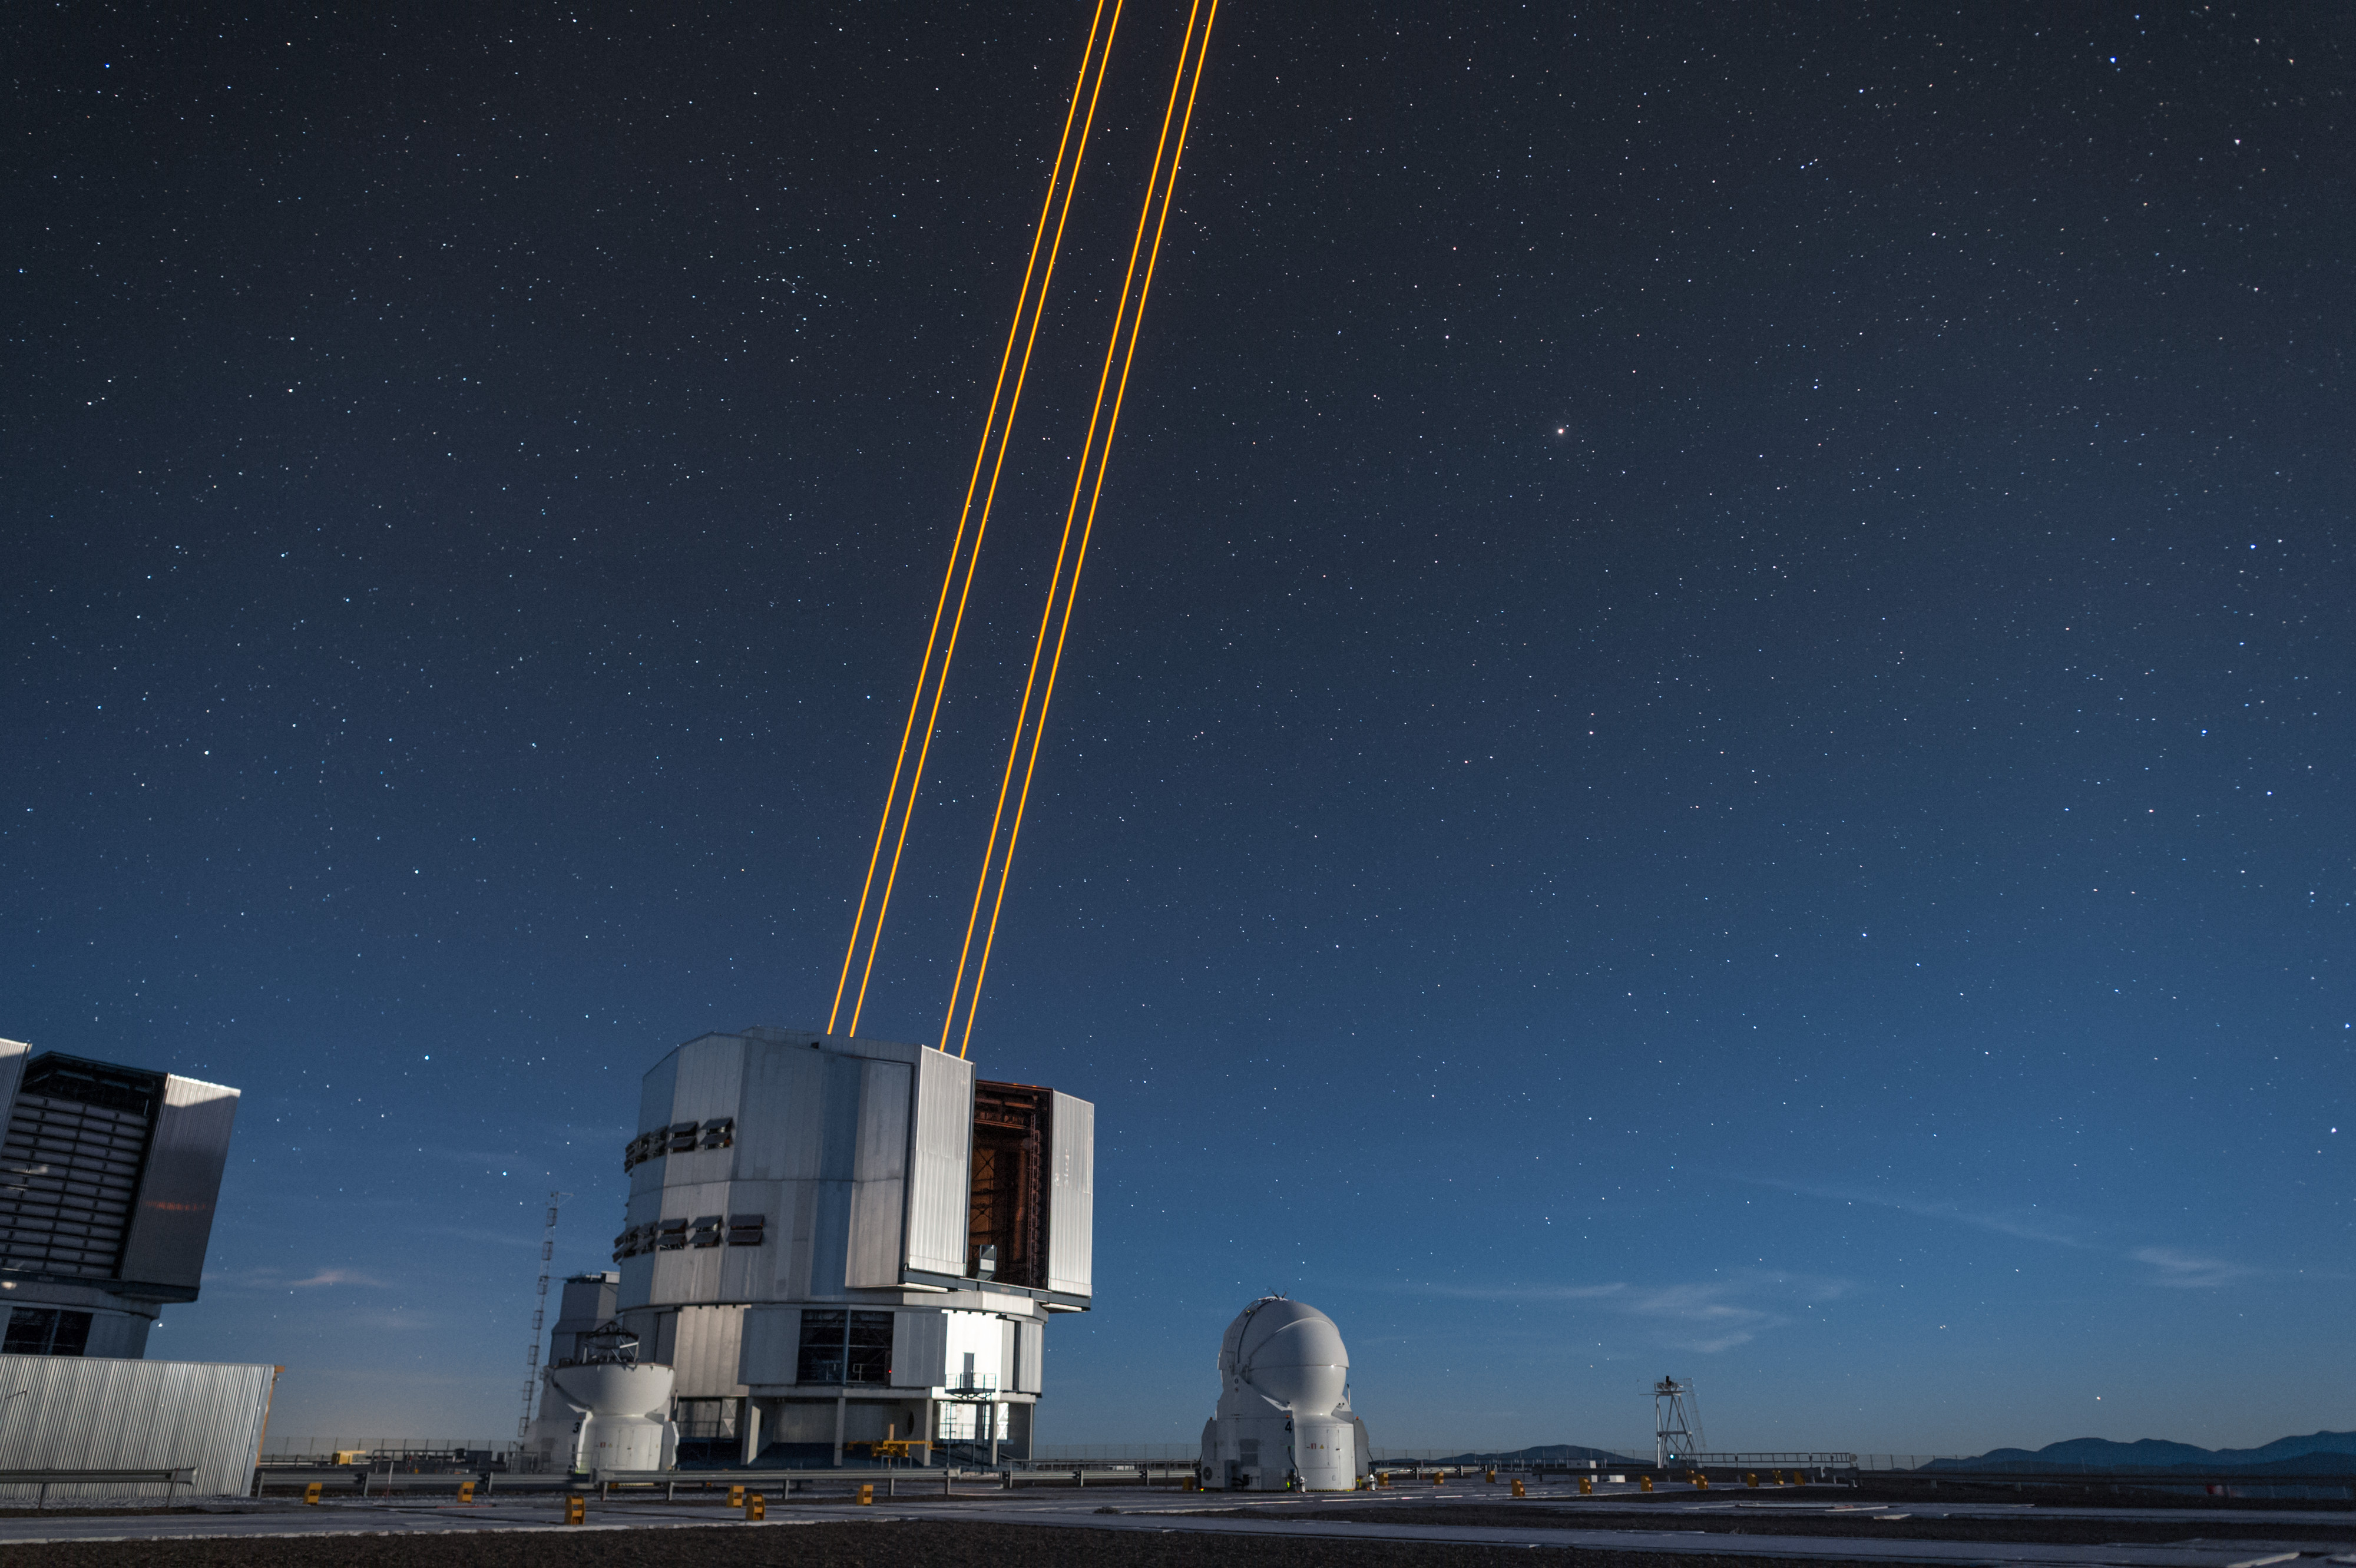
\includegraphics[width=0.5\textwidth]{adaptiv/images/Leitstern}
  \caption{Erzeugung eines Leitsterns (VLT der ESO Paranal Observatorium)
    \cite{eso:leitstern}}
  \label{fig:leitstern}
\end{figure}

\section{Kürzester Weg}
Wenn wir zwei Punkte im Raum betrachten und den kürzesten Weg zwischen ihnen suchen, so würden wir intuitiv die Punkte mit einer Geraden verbinden und diesen Weg als den kürzesten definieren. Wenn nun aber das Licht den kürzesten Weg zwischen zwei Punkten geht, wird nicht wie beim klassischen Weg die Strecke minimiert, sondern die Laufzeit die das Licht benötigt. Das führt dazu, dass wenn zwischen den zwei Punkten eine Phasengrenze liegt, der Weg nicht mehr die direkte Verbindung ist, sondern eine Streckte, die abhängig von Brechungsindex der beiden Phasen einem der möglichen Wege auf der Abbildung \ref{fig:weg} entspricht. Dieses Verhalten wird von Fermat's Prinzip beschrieben, welches sagt dass, das die Laufzeit zwischen den Punkten optimiert wird. Beim suchen des kürzesten Weges, befinden wir uns auf dem Themengebiet der geometrischen Optik, das Licht ist also nur ein Strahl. 
\begin{figure}
  \centering
  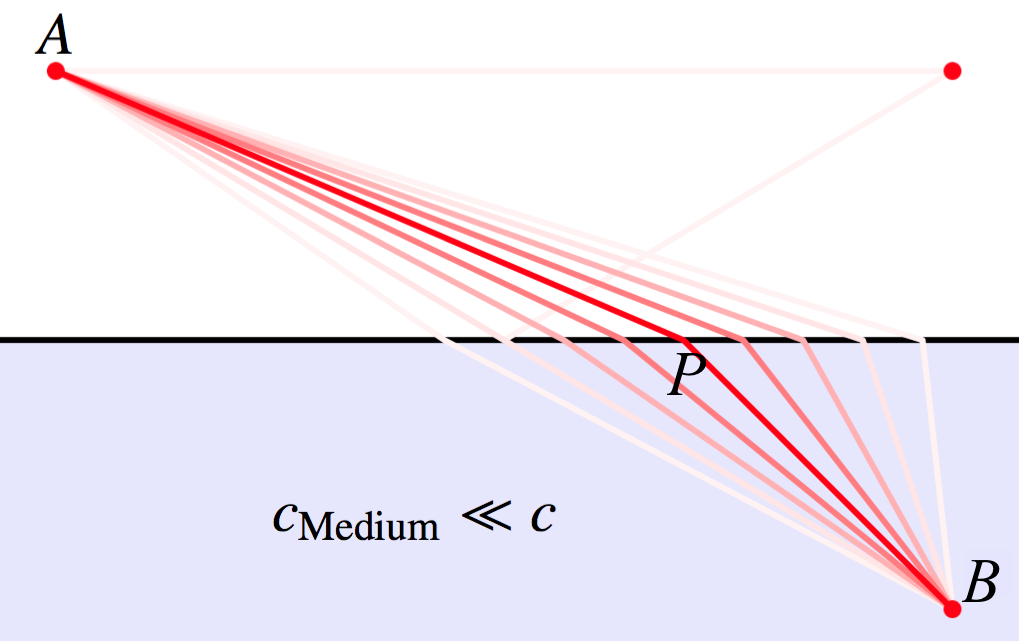
\includegraphics[width=0.5\textwidth]{adaptiv/images/Weg}
  \caption{Kürzester Weg zwischen zwei Punkten}
  \label{fig:weg}
\end{figure}
Welchen Weg nimmt nun aber das Licht, wenn es wie auf der Abbildung \ref{fig:weg} von A nach B muss und dazwischen ein Übergang des Mediums stattfindet, somit das Licht nicht den intuitiv direkten Weg gehen kann. Nach dem Prinzip von Fermat muss also die Zeit auf $\overline{AP}$ und $\overline{PB}$ minimal sein. Die Gleichung \eqref{bedmin} gibt die Bedingung an, mit welcher die Laufzeit vom Licht minimal ist.

\begin{equation}\label{bedmin}
\dfrac{\partial t}{\partial p_{x}}=0
\end{equation}
Um $t$ zu bestimmen werden nun die Strecken $\overline{AP}$ und $\overline{PB}$ benötigt. Dabei haben die Punkte die folgenden Koordinaten $A = (0,a)$, $P=(p_{x},p_{y})$ und $B=(b,0)$. Die Gleichung \eqref{tbest} erklärt, wie aus Abblidung \ref{fig:weg} die jeweiligen Strecken bestimmt werden können. In einem weiteren Schritt wird die Gleichung \eqref{tbest} partiell nach $p_{x}$ abgeleitet und die Ableitung gleich Null gesetzt.

\begin{equation}\label{tbest}
t=\dfrac{s}{s}=\dfrac{\overline{AP}}{v_{1}}+\dfrac{\overline{PB}}{v_{2}}= 
\dfrac{\sqrt{(a-p_{y})^{2}+p_{x}^{2}}}{v_{1}}+ 
\dfrac{\sqrt{(b-p_{x})^{2}+p_{y}^{2}}}{v_{2}}
\end{equation}

\begin{equation}\label{partdiff}
\dfrac{\partial t}{\partial p_{x}}=
\dfrac{1}{v_{1}}\cdot \dfrac{1}{2 \sqrt{(a-p_{y})^{2}+p_{x}^{2}}}\cdot 2p_{x} +
\dfrac{1}{v_{2}}\cdot \dfrac{-1}{2 \sqrt{(b-p_{x})^{2}+p_{y}^{2}}}\cdot 2(b-p_{x})= 0
\end{equation}

\begin{equation}\label{glp}
\dfrac{n_{1}\cdot 2p_{x} }{\sqrt{(a-p_{y})^{2}+p_{x}^{2}}}+
\dfrac{-n_{2}\cdot 2(b-p_{x})}{\sqrt{(b-p_{x})^{2}+p_{y}^{2}}}= 0
\end{equation}

Die Geschwindigkeit $ v_{1}$ ist gleich $\frac{c}{n_{1}} $ und $ v_{2}$ ist gleich $\frac{c}{n_{2}}$, dabei ist $v_{i}$ die Lichtgeschwindigkeit im jeweiligen Medium. Wird nun in die Gleichung \eqref{partdiff} $ v_{1}$ und $ v_{2}$ eingesetzt und anschliessend mit $c$ multipliziert, erhält man die Gleichung \eqref{glp1} aus welchen dann der Punkt $P$ respektive die Koordinate $p_{x}$ von $P$ bestimmt werden kann.
Auf der Abbildung \ref{fig:nullstelle} ist eine grafische Darstellung der der Ableitungen zu sehen, dabei wird der Brechungsindex variiert, die Position des Punktes $P$ auf der Abbildung \ref{fig:weg} verändert seine Position in X-Richtung. Die  Punkte haben dabei die folgenden Koordinaten $A = (0,6)$, $P=(p_{x},3)$ und $B=(10,0)$, für die Situation $n_{1}=n_{2}$ gibt es keine Übergang der Punkt $P$ hat die Koordinaten $(5,3)$ was genau dem direkten Weg entspricht. Mit den geeigneten Hilfsmitteln (Matlab) ist es möglich die Gleichung \eqref{glp} nach $p_{x}$ umzustellen, die Lösung ist aber unübersichtlich und sehr lang, die Abbildung \ref{fig:nullstelle} ist da aussagekräftiger.
Damit ist der Strahlengang von $A$ nach $B$ via $P$ bestimmt. Dieser Weg ist nun minimal bezüglich der Laufzeit. \newline
Zur besseren Verständlichkeit noch eine kleiner Vergleich:\newline
Es ist nun kein Photon das den Weg zurücklegen muss, sondern ein ausgesprochen intelligenter Hund der bei $A$ startet und bei $B$ einen Ball im Wasser holen muss, die schwarz horizontale Linie auf der Abbildung \ref{fig:weg} ist dabei das Ufer. Wenn nun der Hund den zuvor beschrieben Weg wählt, ist er am schnellsten beim Ball. Der Grund dafür ist, er rennt an Land schneller als er schwimmen kann. Der Punkt $P$ ist also der optimale Punkt für den Hund um uns Wasser zu springen.
\begin{figure}
  \centering
  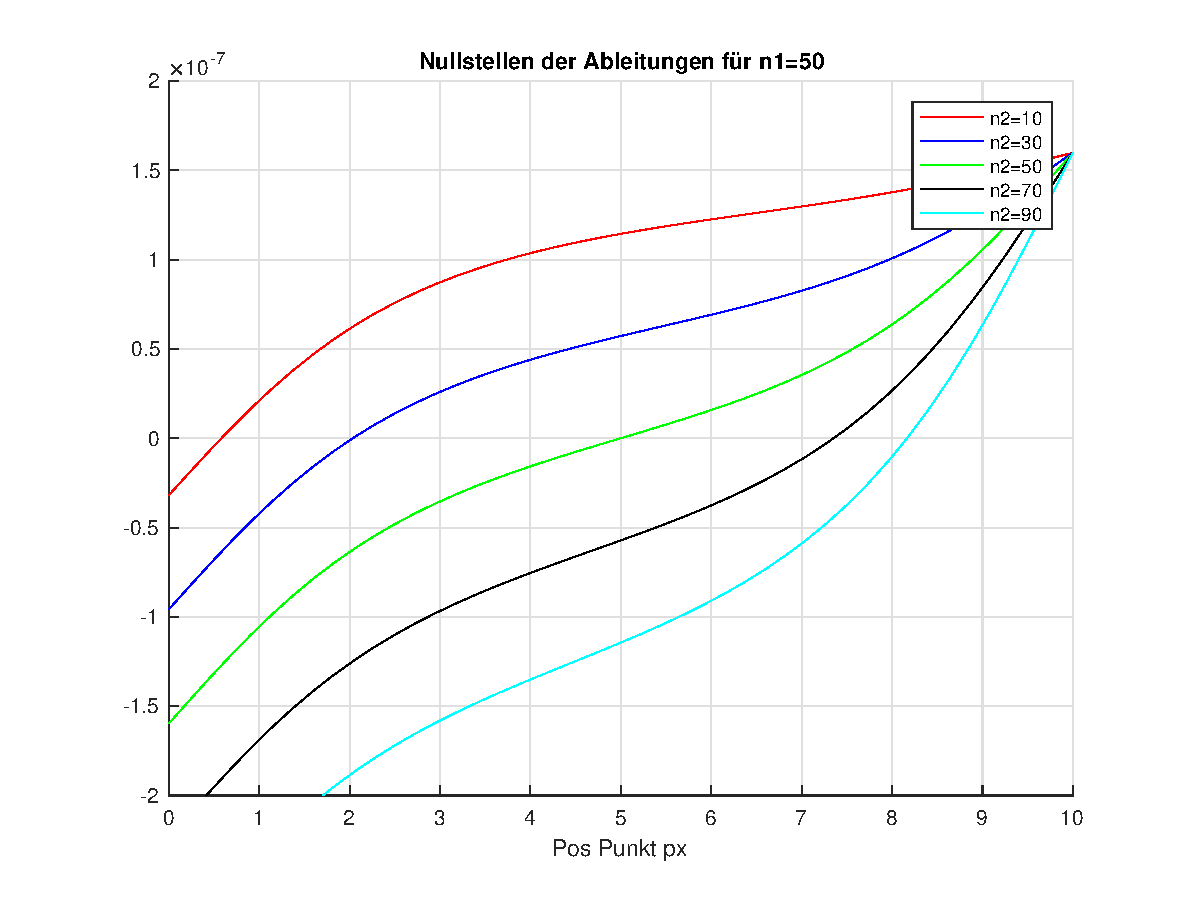
\includegraphics[width=0.5\textwidth]{adaptiv/images/Nullstellen}
  \caption{Nullstellen der Ableitung abhängig vom Brechungsindex}
  \label{fig:nullstelle}
\end{figure}

\subsection{Warum der kürzeste Weg}
Auf dem Weg von der Lichtquelle, in der Astronomie sind das oft Sterne, Sternhaufen, Galaxien oder sogar ganze Cluster von Galaxien, trifft das Licht immer wieder auf Störeinflüsse. Störungen die auf dem Weg durch dass All entstehen werden im nächsten Kapitel besprochen, in diesem Abschnitt geht es ja um Störungen die in der Atmosphäre entstehen. Wenn mit einem Teleskop Sterne beobachtet werden kann man immer von sehr gutem Wetter ausgehen und trotzdem ist die Atmosphäre vielschichtig aufgebaut. Das Licht sucht sich nun den schnellsten Weg durch die verschiedenen Schichten, dabei ist bei jedem Übergang zwischen zwei Schichten auch zu "Richtungsänderung" des Lichtes wie auf Abbildung \ref{fig:weg}.

\section{Wellenfront}
Das Licht von Leitstern, der mit dem Laser erzeugt wird ist nun die Referenzlichtquelle mit welcher die Atmosphärenstörung messen kann, welche das Licht beim passieren der Schicht erfährt. Dabei werden einige Näherungen gemacht, eine davon ist, dass auf der Hartmannplatte mit einer ebenen Wellenfront gerechnet wird, die ist auf der Abbildung \ref{fig:hartmannplatte} schön zu sehen. Der künstliche Leitstern ist aber eigentlich eine kugelförmige Quelle, warum also darf diese Näherung gemacht werden. Die Näherung ist möglich, da der Leitstern 90$km$ vom Sensor entfernt ist, die Krümmung der Wellenfront ist so gering, das sie nur noch eine kleinen Einfluss hat, sie also vernachlässigt werden kann und dadurch die Berechnung vereinfacht wird. Im Kapitel 4 wird das Thema der Krümmung behandelt, als kleine Anwendung wird im folgenden Abschnitt die Krümmung der kugelförmigen Welle berechnet.

\subsection{Krümmung der Wellenfront}
Die Wellenfront wird durch die Funktion \eqref{kugelfunktion} beschrieben. Davon muss nun die Krümmung berechnet werden, um den Fehler durch die Näherung bestimmen zu können. Korrekterweise müsste vor der Wurzen noch $\pm$ stehen, da sonst nur die obere Hälfte der Kugel betrachtet wird, da wir aber nur an der Krümmung der Kugel interessiert sind und die auf der ganzen Kugel gleich ist, kann dieses $\pm$ weggelassen werden.
\begin{equation}\label{kugelfunktion}
z=f(x,y)=\sqrt{r^{2}-x^{2}-y^{2})}
\end{equation}
Es um die gausssche Krümmung zu berechnen, werden die ersten und zweiten partiellen Ableitungen und die Ableitung $ \frac{df}{dxdy}$ benötigt.

\begin{equation}\label{Ableitungen x}
f_{x}=\dfrac{\partial f(x,y)}{\partial x}= \dfrac{-x}{\sqrt{r^{2}-x^{2}-y^{2}}}
\end{equation}

\begin{equation}\label{Ableitungen xx}
f_{xx}=\dfrac{\partial f(x,y)}{\partial x^{2}}= \dfrac{- x^2}{(r^2 - x^2 - y^2)^{\frac{2}{3}}}+\dfrac{ - 1}{(r^2 - x^2 - y^2)^{\frac{1}{2}}}
\end{equation}

\begin{equation}\label{Ableitungen y}
f_{y} =\dfrac{\partial f(x,y)}{\partial x}= \dfrac{-y}{\sqrt{r^{2}-x^{2}-y^{2}}}
\end{equation}

\begin{equation}\label{Ableitungen yy}
f_{yy}=\dfrac{\partial f(x,y)}{\partial y^{2}}= \dfrac{- x^2}{(r^2 - x^2 - y^2)^{\frac{2}{3}}}+\dfrac{ - 1}{(r^2 - x^2 - y^2)^{\frac{1}{2}}}
\end{equation}

\begin{equation}\label{Ableitungen xy}
f_{xy}=\dfrac{\partial f(x,y)}{\partial x \partial y}=  \dfrac{-xy}{\sqrt{r^{2}-x^{2}-y^{2}}}
\end{equation}
Die Herleitung der Krümmung und die entsprechenden Beweise dazu sind im Kapitel 4 zu finden. Die gaussche Krümmung lässt sich berechnen, in dem man die Gleichungen \eqref{Ableitungen x} bis \eqref{Ableitungen xy} in die Gleichung \eqref{gausskrümmung} einsetzt.  

\begin{equation}\label{gausskrümmung}
h = \dfrac{f_{xx} \cdot f_{yy} -f_{xy}^{2}}{(1+f_{x}^{2}+f_{y}^{2})^{2}} = \dfrac{1}{r^{2}} =\dfrac{1}{90000^{2}} = 1.234\cdot 10^{-10}
\end{equation}
Nach dem einsetzen und vereinfachen der Gleichung \eqref{gausskrümmung} bekommt man die den sehr einfachen Ausdruck $\frac{1}{r^{2}}$ für die Krümmung der Kugeloberfläche. Wie zu erwarten war, ist die Krümmung der nicht von der Position auf der Kugel abhängigd. 
Der daraus Berechnete Wert ist mit $1.234\cdot 10^{-10}$ so klein, dass die Krümmung der Wellenfront vernachlässigt werden darf, ohne dass die Qualität der adaptiven Optik sich merklich verändert.



\printbibliography[heading=subbibliography]
\end{refsection}














